\documentclass[a4paper, 12pt]{article}
\usepackage[utf8]{inputenc}
\usepackage[russian,english]{babel}
\usepackage[T2A]{fontenc}
\usepackage[left=10mm, top=20mm, right=10mm, bottom=15mm, footskip=13mm]{geometry}
\usepackage{indentfirst}
\usepackage{amsmath,amssymb}
\usepackage{graphicx}
\usepackage[italicdiff]{physics}
\usepackage{float}
\usepackage{array}
\usepackage{physics}
\graphicspath{ {shema/} {graphic/} }
\usepackage{caption}
\captionsetup[figure]{name=Рисунок}
  
\title{Отчет по лабораторной работе 1.2.5

Исследование вынужденной регулярной прецессии гироскопа}

\author{Максим Осипов, Б03-504}
\date{22.10.2025}

\begin{document}
\maketitle

\section{Аннотация}

\textbf{Цель работы:} исследовать вынужденную прецессию гироскопа, установить зависимость скорости вынужденной прецессии от величины момента сил, действующий на ось гироскопа и сравнить ее со скоростью, рассчитанной по скорости прецессии.\\
\textbf{Оборудование:} гироскоп в кардановом подвесе, секундомер, набор грузов, отдельный ротор гироскопа, цилиндр известной массы, крутильный маятник, штангенсциркуль, линейка.

\section{Теоретическая справка}
Движение твердого тела описывается двумя векторными уравнениями:
\begin{align}
\frac{d\vec{P}}{dt} &= \vec{F}, \\
\frac{d\vec{L}}{dt} &= \vec{M}.
\end{align}
Уравнение (1) выражает закон движения центра масс тела, а уравнение (2) — уравнение моментов. Этих уравнений достаточно для полного описания движения твердого тела, имеющего шесть степеней свободы.

Момент импульса твердого тела в его главных осях $x$, $y$, $z$ равен
\begin{equation}
\vec{L} = \vec{i} I_x \omega_x + \vec{j} I_y \omega_y + \vec{k} I_z \omega_z,
\end{equation}
где $I_x$, $I_y$, $I_z$ — главные моменты инерции, $\omega_x$, $\omega_y$, $\omega_z$ — компоненты вектора угловой скорости.

Быстро вращающееся тело, для которого выполнено условие $I_z \omega_z \gg I_x \omega_x, I_y \omega_y$, называют гироскопом. При кратковременном действии момента внешних сил приращение момента импульса мало:
\begin{equation}
|\Delta \vec{L}| \ll |\vec{L}|,
\end{equation}
что объясняет устойчивость быстро вращающегося гироскопа.

\begin{figure}[h]
\centering
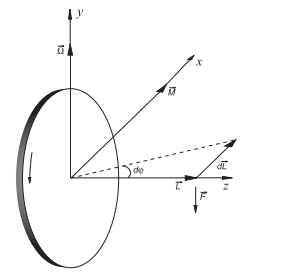
\includegraphics[width=0.4\textwidth]{рис1.png}
\caption{маховик}
\label{fig1}
\end{figure}

Рассмотрим маховик (рис. \ref{fig1}), вращающийся вокруг оси $z$ с $\omega_z = \omega_0$. При повороте оси на малый угол $d\varphi = \Omega dt$ и условии $L_\Omega \ll L_{\omega_0}$ изменение момента импульса:
\begin{equation}
|d\vec{L}| = L d\varphi = L \Omega dt.
\end{equation}

Это изменение направлено вдоль оси $x$ и может быть представлено как векторное произведение:
\begin{equation}
d\vec{L} = \vec{\Omega} \times \vec{L} dt,
\end{equation}
откуда
\begin{equation}
\frac{d\vec{L}}{dt} = \vec{\Omega} \times \vec{L}.
\end{equation}

С учетом уравнения моментов (2) получаем основное уравнение прецессии:
\begin{equation}
\vec{M} = \vec{\Omega} \times \vec{L}.
\end{equation}

Под действием момента $\vec{M}$ ось гироскопа вращается с постоянной угловой скоростью $\vec{\Omega}$ — такое движение называется регулярной прецессией.

\begin{figure}[h]
\centering
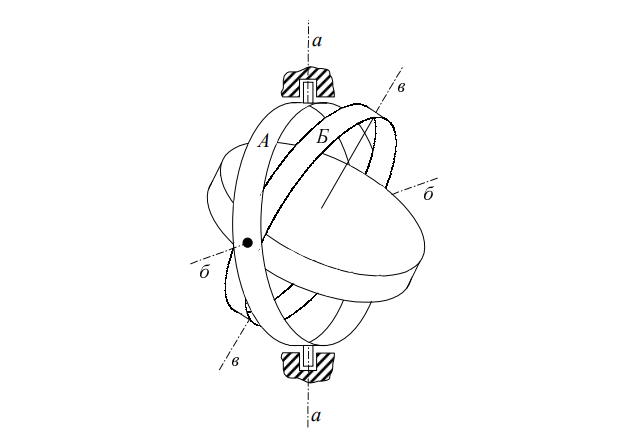
\includegraphics[width=0.7\textwidth]{рис2.png}
\caption{Гироскоп в кардановом подвесе}
\label{fig2}
\end{figure}

Для гироскопа в кардановом подвесе (рис. \ref{fig2}) массой $m_r$, наклоненного на угол $\alpha$, скорость прецессии под действием силы тяжести:
\begin{equation}
\Omega = \frac{M}{I_z \omega_0 \sin \alpha} = \frac{m_r g l_{u} \sin \alpha}{I_z \omega_0 \sin \alpha} = \frac{m_r g l_{u}}{I_z \omega_0},
\end{equation}
где $l_u$ — расстояние от точки подвеса до центра масс.

При подвешивании дополнительного груза массой $m$:
\begin{equation}
\Omega = \frac{mgl}{I_z\omega_0},
\end{equation}
где $l$ — расстояние от центра подвеса до точки крепления груза.

\begin{figure}[h]
\centering
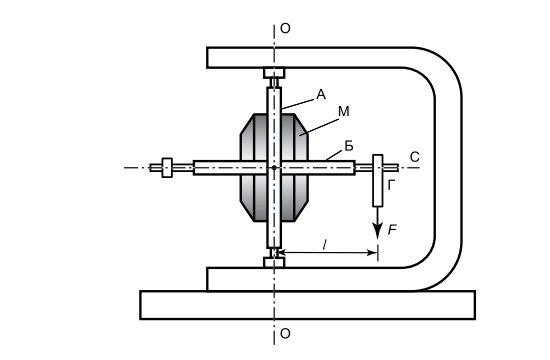
\includegraphics[width=0.6\textwidth]{рис3.png}
\caption{Экспериментальная установка}
\label{fig3}
\end{figure}

Момент инерции ротора $I_0$ определяют по крутильным колебаниям (рис. \ref{fig3}). Период колебаний:
\begin{equation}
T_0 = 2\pi\sqrt{\frac{I_0}{f}}.
\end{equation}

Используя эталонный цилиндр с известным моментом инерции $I_u$:
\begin{equation}
I_0 = I_u\frac{T_0^2}{T_u^2},
\end{equation}
где $T_u$ — период колебаний цилиндра.

Скорость вращения ротора измеряют по ЭДС индукции во второй обмотке статора. Ротор электромотора намагничен и при вращении наводит переменную ЭДС, частоту которой измеряют по фигурам Лиссажу на осциллографе.

Силы трения в осях карданова подвеса не лежат в плоскости осей вращения и вызывают опускание оси гироскопа, что необходимо учитывать при проведении измерений.
\end{document}
